\section{The Cross Product} \label{S:9.4.Cross_Product}

\vspace*{-14 pt}
\framebox{\hspace*{3 pt}
\parbox{6.25 in}{\begin{goals}
  \item How and when is the cross product of two vectors defined?
  \item What geometric information does the cross product provide?
\end{goals}} \hspace*{3 pt}}

The last two sections have introduced some basic algebraic operations
on vectors---addition, scalar multiplication, and the dot
product---with useful geometric interpretations.  In
this section, we will meet a final algebraic operation, the {\em cross
  product}, which again conveys important geometric information.

To begin, we must emphasize that the cross product is only defined for
vectors $\vu$ and $\vv$ in $\R^3$.  
Also, remember that we use a right-hand coordinate
system, as described in Section \ref{S:9.1.Functions}.  In
particular, recall that the vectors $\vi$, $\vj$, and $\vk$ are
oriented as shown below in Figure \ref{F:9.4.basis}.  Earlier, we
noticed that if we point the index finger of our {\em right} hand in
the direction of $\vi$ and our middle finger in the direction of
$\vj$, then our thumb points in the direction of $\vk$.

\begin{figure}[ht]
  \begin{center}
    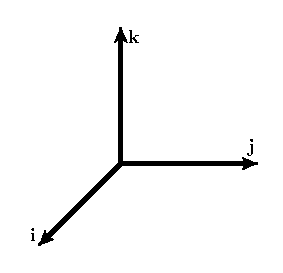
\includegraphics{figures/fig_9_4_basis.eps}
    \caption{Basis vectors $\vi$, $\vj$, and $\vk$.}
    \label{F:9.4.basis}
  \end{center}
\end{figure}

\begin{pa} \label{PA:9.4} 

  The cross product of two vectors, $\vu$ and $\vv$, will itself be a
  {\em vector} denoted $\vu\times\vv$.  The direction of
  $\vu\times\vv$ is determined by the right-hand rule: if we point the
  index finger of our right hand in the direction of $\vu$ and our
  middle finger in the direction of $\vv$, then our thumb points in
  the direction of $\vu\times\vv$.

  \ba

  \item We begin by defining the cross products using the vectors $\vi$,
  $\vj$, and $\vk$.  Referring to Figure \ref{F:9.4.basis}, explain
  why $\vi$, $\vj$, $\vk$ in that order form a right-hand system. We then define $\vi \times \vj$ to be $\vk$ -- that is $\vi\times\vj = \vk$.  
  \item Now explain why $\vi$, $\vk$, and $-\vj$ in that order form a right-hand system. We then define $\vi \times \vk$ to be $-\vj$ -- that is  $\vi\times\vk=-\vj$.
  \item Continuing in this way, complete the missing entries in Table~\ref{T:9.4.cross.def}.
    \begin{table}[ht]
      \begin{center}
        \begin{tabular}{lll}
          $\vi\times\vj = \vk$ \hspace*{1in} &
          $\vi\times\vk = -\vj$ \hspace*{1in} &
          $\vj\times\vk = $\hspace*{1in} \\ \\
          $\vj\times\vi = $ &
          $\vk\times\vi = $ &
          $\vk\times\vj = $
        \end{tabular}
      \end{center}
      \caption{Table of cross products involving $\vi$, $\vj$, and $\vk$.} 
      \label{T:9.4.cross.def}
    \end{table}

  \item Up to this point, the products you have seen, such as the
    product of real numbers and the dot product of vectors, have been
    commutative, meaning that the product does not depend on the order
    of the terms.  For instance, $2\cdot5 = 5\cdot 2$.  The table
    above suggests, however, that the cross
    product is {\em anti-commutative}: for any vectors $\vu$ and $\vv$ in $\R^3$,  $\vu\times\vv =
    -\vv\times\vu$.  

    If we consider the case when $\vu=\vv$, this shows that
    $\vv\times\vv = -\vv\times\vv$.  What does this tell us about
    $\vv\times\vv$;  in particular, what vector is unchanged by
    scalar multiplication by $-1$?

  \item The cross product is also a {\em bilinear} operation, meaning
    that it interacts with scalar multiplication and vector addition
    as one would expect:  
    $(c\vu + \vv)\times\vw = c(\vu\times\vw) + \vv\times\vw$. For example, 
\[(2\vi + \vj) \times \vk = 2(\vi \times \vk) + (\vj \times \vk) = -2\vj + \vi.\]
Using this property along with Table~\ref{T:9.4.cross.def}, find the cross product $\vu\times\vv$ if
    $\vu = 2\vi + 3\vj$ and $\vv = -\vi + \vk$.

  \item Verify that the cross product $\vu\times\vv$ you just found in
    part (e) is
    orthogonal to both $\vu$ and $\vv$.

  \item Consider the vectors $\vu$ and $\vv$ in the $xy$-plane as
    shown below in Figure \ref{F:9.4.activity_1}.

    \begin{figure}[ht]
      \begin{center}
        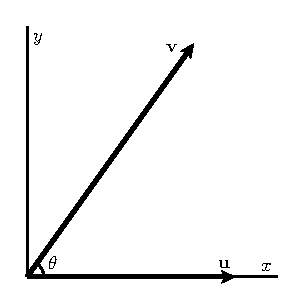
\includegraphics{figures/fig_9_4_activity_1.eps}
        \caption{Two vectors in the $xy$-plane}
        \label{F:9.4.activity_1}
      \end{center}
    \end{figure}

    Explain why $\vu = |\vu|\vi$ and $\vv = |\vv|\cos\theta \vi +
    |\vv|\sin\theta \vj$.  Then compute the length of $|\vu\times\vv|$.

  \item Multiplication of real numbers is {\em associative}, which
    means, for instance, that $(2\cdot 5)\cdot 3 = 2\cdot(5\cdot 3)$.
    Is it true that the cross product of vectors is associative?  For
    instance, is it true that
    $(\vi\times\vj)\times\vj = \vi\times(\vj\times\vj)$?

    \ea




\end{pa} 

\begin{activitySolution}
  \ba

  \item If we point the index finger of our right hand in the direction of $\vi$ and our middle finger in the direction of $\vj$, then our thumb points in the direction of $\vk$. So $\vi$, $\vj$, and $\vk$ form a right hand system.  
  \item If we point the index finger of our right hand in the direction of $\vi$ and our middle finger in the direction of $\vk$, then our thumb points in the opposite direction of $\vj$. So $\vi$, $\vk$, and $-\vj$ form a right hand system. 
  \item The cross products of combinations of the standard unit vectors are shown in the figure below. 
%   \begin{table}[ht]
     \begin{center}
       \begin{tabular}{lll}
          $\vi\times\vj = \vk$ \hspace*{1in} &
          $\vi\times\vk = -\vj$ \hspace*{1in} &
          $\vj\times\vk = \vi$\hspace*{1in} \\ \\
          $\vj\times\vi = -\vk$ &
          $\vk\times\vi = \vj$ &
          $\vk\times\vj = -\vi$
       \end{tabular}
      \end{center}
%      \caption{Table of cross products involving $\vi$, $\vj$, and $\vk$.} 
 %     \label{T:9.4.cross.def_sol}
 %  \end{table}

  \item The only vector that is unchanged by scalar multiplication by $-1$ is the zero vector. So we conclude that $\vv \times \vv = \vzero$. 

  \item Using the bilinearity of the cross product we find that 
  \begin{align*}
\vu \times \vv &= (2\vi + 3\vj) \times (-\vi + \vk) \\
	&= -2(\vi \times \vi) + 2(\vi \times \vk) - 3 (\vj \times \vi) + 3(\vj \times \vk) \\
	&= -2 \vzero - 2\vj +3 \vk + 3\vi \\
	&= 3 \vi - 2 \vj + 3 \vk.
\end{align*}

  \item Recall that two nonzero vectors are orthogonal if their dot product is 0. Since 
\[\vu \cdot (\vu \times vv) = (2 \vi + 3 \vj) \cdot (3 \vi - 2 \vj + 3 \vk) = 6 - 6 = 0\]
and
\[\vv \cdot (\vu \times vv) = (- \vi +  \vk) \cdot (3 \vi - 2 \vj + 3 \vk) = -3 + 3 = 0,\]
it follows that $\vu \times \vv$ is orthogonal to both $\vu$ and $\vv$. 

  \item Since $\vu$ is parallel to $\vi$, it must be the case that $\vu$ is a scalar multiple of $\vi$. Now $\vi$ is a unit vector and the magnitude of $\vu$ is $|\vu|$, so $\vu = |\vu| \vi$. The vector $\vv$ forms the hypotenuse of a right triangle with the $x$-axis as base. The horizontal leg of this triangle is the vector $|\vv| \cos(\theta) \vi$ and the vertical leg is the vector $|\vv|\sin(\theta) \vj$. Geometrically, we can see that vector legs sum to the vector hypotenuse, so $\vv = |\vv| \cos(\theta) \vi + |\vv| \sin(\theta) \vj$. Then
\begin{align*}
|\vu \times \vv| &= |(|\vu| \vi) \times (|\vv| \cos(\theta) \vi + |\vv| \sin(\theta) \vj) | \\
	&=  ||\vu| |\vv| \cos(\theta) (\vi \times \vi) + |\vu| |\vv| \sin(\theta) (\vi \times \vj) | \\
	&= ||\vu| |\vv| \sin(\theta) \vk | \\
	&= |\vu| |\vv| |\sin(\theta) |. 
\end{align*}

  \item Note $(\vi\times\vj)\times\vj = \vk \times \vj = -\vi$ while $\vi\times(\vj\times\vj) = \vi \times \vzero = \vzero$. So the cross product is not an associative operation. 
    \ea

\end{activitySolution}

\afterpa 

\subsection*{Computing the cross product}

As we have seen in Preview Activity \ref{PA:9.4}, the cross product
$\vu\times\vv$ is defined for two vectors $\vu$ and $\vv$ in $\R^3$
and produces another vector in $\R^3$.
Using the right-hand rule, we saw that

\begin{table}[ht]
  \label{T:9.4.cross.basis}
  \begin{center}
    \begin{tabular}{lll}
      $\vi\times\vj = \vk,$ \hspace*{1in} &
      $\vi\times\vk = -\vj,$ \hspace*{1in} &
      $\vj\times\vk = \vi$\hspace*{1in} \\ \\
      $\vj\times\vi = -\vk$ &
      $\vk\times\vi = \vj$ &
      $\vk\times\vj = -\vi$
    \end{tabular}
  \end{center}
\end{table}

If in addition we apply the bilinearity property to compute the cross product
in terms of the components of general vectors, $\vu$ and $\vv$ we see that\footnote{Like the dot product, the cross product arises in physical applications, e.g., torque, but is it more convenient mathematically to begin from an algebraic perspective.} 
\begin{eqnarray*}
  \vu\times\vv & = & (u_1\vi + u_2\vj + u_3\vk) \times 
  (v_1\vi + v_2\vj + v_3\vk) \\
  & = & u_1\vi\times  (v_1\vi + v_2\vj + v_3\vk)+ \\
  & & u_2\vj\times  (v_1\vi + v_2\vj + v_3\vk)+ \\
  & & u_3\vk\times  (v_1\vi + v_2\vj + v_3\vk) \\
  & = & u_1v_1\vi\times\vi + u_1v_2\vi\times\vj + u_1v_3\vi\times\vk +\\
  &  & u_2v_1\vj\times\vi + u_2v_2\vj\times\vj + u_2v_3\vj\times\vk + \\
  &  & u_3v_1\vk\times\vi + u_3v_2\vk\times\vj + u_3v_3\vk\times\vk
  \\
  & = & u_1v_2\vk - u_1v_3\vj - u_2v_1\vk + u_2v_3\vi +u_3v_1\vj -
  u_3v_2\vi \\
  & = & (u_2v_3-u_3v_2)\vi - (u_1v_3-u_3v_1)\vj + (u_1v_2-u_2v_1)\vk
\end{eqnarray*}
To summarize, we have shown that
\begin{equation}\label{E:9.4.cross.def}
(u_1\vi + u_2\vj + u_3\vk) \times 
  (v_1\vi + v_2\vj + v_3\vk) = 
(u_2v_3-u_3v_2)\vi - (u_1v_3-u_3v_1)\vj + (u_1v_2-u_2v_1)\vk.
\end{equation}

At first, this may look intimidating and difficult
to remember.  However, if we rewrite the expression in Equation~\eqref{E:9.4.cross.def} using determinants, 
important structure emerges.  The determinant of a $2\times2$ matrix is
$$
\left|
  \begin{array}{cc}
    a & b \\
    c & d 
  \end{array}
\right|
=ad - bc.$$
It follows that we can thus rewrite Equation~\eqref{E:9.4.cross.def} in the form
$$
\vu\times\vv = 
\left|
  \begin{array}{cc}
    u_2 & u_3 \\
    v_2 & v_3 \\
  \end{array}
\right| \vi
-
\left|
  \begin{array}{cc}
    u_1 & u_3 \\
    v_1 & v_3 \\
  \end{array}
\right| \vj
+
\left|
  \begin{array}{cc}
    u_1 & u_2 \\
    v_1 & v_2 \\
  \end{array}
\right| \vk.
$$
For those familiar with the determinant of a $3\times3$ matrix, we
write the mnemonic
$$
\vu\times\vv = 
\left|
  \begin{array}{ccc}
    \vi & \vj & \vk \\
    u_1 & u_2 & u_3 \\
    v_1 & v_2 & v_3
  \end{array}
\right|.
$$

\newpage
\begin{activity} \label{A:9.4.5}  Suppose 
  $\vu = \langle 2, -1, 0\rangle$ and $\vv = \langle 0, 1, 3\rangle$.
  Use the formula (\ref{E:9.4.cross.def}) for the following.
  \ba
  \item Find the cross product $\vu\times\vv$.  

  \item Find the cross product $\vu\times \vi$.

  \item Find the cross product $\vu\times\vu$.

  \item Evaluate the dot products $\vu\cdot(\vu\times\vv)$ and
    $\vv\cdot(\vu\times\vv)$.  What does this tell you about the
    geometric relationship among $\vu$, $\vv$, and $\vu\times\vv$?

    \ea
\end{activity}

\begin{activitySolution}
\ba
	\item By the formula we have
\[\langle 2, -1, 0\rangle \times \langle 0, 1, 3\rangle = ((-1)(3)-0) \vi - ((2)(3)-0)\vj + ((2)(1)-0)\vk = -3 \vi - 6\vj + 2\vk.\]

	\item By the formula we have
\[\langle 2, -1, 0\rangle \times \langle 1, 0, 0\rangle = (0) \vi - (0)\vj + (0-(-1)(1))\vk = \vk.\] 

	\item By the formula we have
\[\langle 2, -1, 0\rangle \times \langle 2, -1, 0\rangle = (0) \vi - (0)\vj + (-2-(-2))\vk = \vzero.\] 

	\item Using the definition of the dot product we have
	\begin{align*}
	\vu\cdot(\vu\times\vv) &= \langle 2, -1, 0\rangle \cdot \langle -3, -6, 2 \rangle = 0 \\
	\vv\cdot(\vu\times\vv) &= \langle 0, 1, 3\rangle \cdot \langle -3, -6, 2 \rangle = 0.
	\end{align*}
So both $\vu$ and $\vv$ are perpendicular to $\vu\times\vv$. 
	\ea
\end{activitySolution}

\aftera


The cross product satisfies the following properties, which were
illustrated in Preview Activity \ref{PA:9.4} and may be easily
verified from the definition (\ref{E:9.4.cross.def}).

\vspace*{5pt}
\nin 
\framebox{
  \hspace*{3 pt}
  \parbox{6.25 in}{
    Let $\vu$, $\vv$, and $\vw$ be vectors in $\R^3$, and
    let $c$ be a scalar. Then 
    \begin{enumerate}
    \item $\vu \times \vv = -(\vv \times \vu)$
    \item $(c\vu +\vv)\times \vw = c(\vu \times \vw) + \vv \times \vw$
    \item $\vu\times\vv = \vzero$ if $\vu$ and $\vv$ are parallel.
    \item The cross product is not associative;  that is, in general
      $$(\vu\times\vv)\times\vw \neq \vu\times(\vv\times\vw).$$
    \end{enumerate}
  } 
  \hspace*{3 pt}
}
\vspace*{5pt}

Just as we found for the dot product, the cross product provides us
with useful geometric information.  In particular, both the length and
direction of the cross product $\vu\times\vv$ encode information about
the geometric relationship between $\vu$ and $\vv$.

\subsection*{The Length of $\vu\times\vv$}

We may ask whether the length $|\vu\times\vv|$ has any relationship to
the lengths of $\vu$ and $\vv$.  To investigate, we will compute the
square of the length $|\vu\times\vv|^2$ and denote by $\theta$ the
angle between $\vu$ and $\vv$, as in Section \ref{S:9.3.Dot_Product}.
Doing so, we find through some significant algebra that

\begin{eqnarray*}
  |\vu\times\vv|^2&=&(u_2v_3-u_3v_2)^2 + (u_1v_3-u_3v_1)^2 +
  (u_1v_2-u_2v_1)^2 \\
  &=&
  u_2^2 v_3^2- 2u_2u_3v_2v_3 +u_3^2v_2^2 +
  u_1^2 v_3^2 -2u_1u_3v_1v_3 +u_3^2v_1^2 +
  u_1^2 v_2^2 -2u_1u_2v_1v_2 +u_2^2v_1^2 \\
  &=&
  u_1^2(v_2^2+v_3^2) + u_2^2(v_1^2+v_3^2) + u_3^2(v_1^2+v_2^2) -
  2(u_1u_2v_1v_2 + u_1u_3v_1v_3 + u_2u_3v_2v_3) \\
  & = & 
  u_1^2(v_1^2+v_2^2+v_3^2) + u_2^2(v_1^2+v_2^2+v_3^2) +
  u_3^2(v_1^2+v_2^2+v_3^2) - \\
  & &
  (u_1^2v_1^2 + u_2^2v_2^2 + u_3^2v_3^2  + 
  2(u_1u_2v_1v_2 + u_1u_3v_1v_3 + u_2u_3v_2v_3)) \\
  &=&
  (u_1^2+u_2^2+u_3^2)(v_1^2+v_2^2+v_3^2)-(u_1v_1+u_2v_2+u_3v_3)^2  \\
  &=&
  |\vu|^2|\vv|^2-(\vu\cdot\vv)^2 \\
  &=&
  |\vu|^2|\vv|^2(1-\cos^2\theta) \\
  &=&|\vu|^2|\vv|^2\sin^2\theta. \\
\end{eqnarray*}
Therefore, we have found $|\vu\times\vv|^2 = |\vu|^2|\vv|^2\sin^2\theta$,
which means that
\begin{equation}
  \label{E:9.4.cross.length}
  |\vu\times\vv| = |\vu||\vv|\sin\theta.
\end{equation}
 Note that the third property stated above says that $\vu\times\vv = \vzero$ if
$\vu$ and $\vv$ are parallel.  This is reflected in
Equation~(\ref{E:9.4.cross.length}) since $\sin\theta=0$ if $\vu$ and $\vv$ are
parallel, which implies that $\vu\times\vv = \vzero$.

Equation (\ref{E:9.4.cross.length}) also has a geometric implication.
Consider the parallelogram formed by two vectors $\vu$ and $\vv$, as
shown in Figure \ref{F:9.4.area}.  

\begin{figure}[ht]
  \begin{center}
    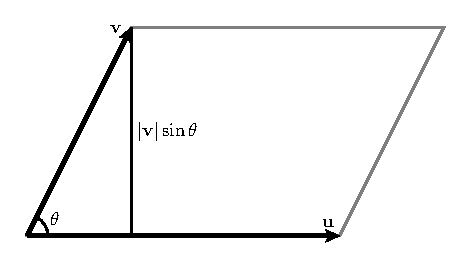
\includegraphics{figures/fig_9_4_area.eps}
    \caption{The parallelogram formed by $\vu$ and $\vv$}
    \label{F:9.4.area}
  \end{center}
\end{figure}


Remember that the area of a parallelogram is the product of its
base and height.  As shown in the figure, we may consider the base of
the parallelogram to be $|\vu|$ and the height to be
$|\vv|\sin\theta$.  This means that the area of the parallelogram
formed by $\vu$ and $\vv$ is 
$$
|\vu||\vv|\sin\theta = |\vu\times\vv|.
$$
This leads to the following interesting fact.

\vspace*{5pt}
\nin \framebox{\hspace*{3 pt}
\parbox{6.25 in}{
  The length, $|\vu \times \vv|$, of the cross product of vectors $\vu$
  and $\vv$ is the area of the parallelogram determined by $\vu$
  and $\vv$.  
} \hspace*{3 pt}} \vspace*{5pt}

\begin{activity} \label{A:9.4.4}  
  \ba
  \item Find the area of the parallelogram formed by the vectors $\vu
    = \langle 1,3, -2\rangle$ and $\vv=\langle 3,0,1\rangle$.
  \item Find the area of the parallelogram in $\R^3$ whose vertices
    are $(1,0,1)$, $(0,0,1)$, 
    $(2,1,0)$, and $(1,1,0)$. 
    \ea
\end{activity}
\begin{smallhint}

\end{smallhint}
\begin{bighint}

\end{bighint}
\begin{activitySolution}
\ba
\item We just need to calculate $|\vu \times \vv|$:
\[|\vu \times \vv| = |\langle 3, -7, -9 \rangle| = \sqrt{139}.\]

\item Let $P=(1,0,1)$, $Q=(0,0,1)$, $R=(2,1,0)$, and $S=(1,1,0)$. Two vectors that determine this parallelogram in $\R^3$ are the vectors 
\[\overrightarrow{PQ} = \langle -1, 0, 0 \rangle = -\vi\]
and 
\[\overrightarrow{PR} = \langle 1, 1, -1 \rangle = \vi + \vj - \vk.\]
Now
\begin{align*}
\overrightarrow{PQ} \times \overrightarrow{PR} &= -\vi \times (\vi+\vj-\vk) \\
	&= -[(\vi \times \vi) + (\vi \times \vj) - (\vi \times \vk)] \\
	&= -[0 + \vk + \vj] \\
	&= \langle 0, -1, -1 \rangle.
\end{align*}
So the area of the parallelogram determined by $\overrightarrow{PQ}$ and $\overrightarrow{PR}$ is 
\[|\overrightarrow{PQ} \times \overrightarrow{PR}| = |\langle 0, -1, -1 \rangle| = \sqrt{2}.\]
\ea

\end{activitySolution}
\aftera



\subsection*{The Direction of $\vu\times\vv$}

Now that we understand the length of $\vu\times\vv$, we will
investigate its direction.  Remember from Preview Activity
\ref{PA:9.4} that cross products involving the vectors $\vi$, $\vj$,
and $\vk$ resulted in vectors that are orthogonal to the two terms.
We will see that this holds more generally.

We begin by computing $\vu\cdot(\vu\times\vv)$, and see that
\begin{eqnarray*}
  \vu\cdot(\vu\times\vv)&=&u_1(u_2v_3-u_3v_2) - u_2(u_1v_3-u_3v_1) +
  u_3(u_1v_2-u_2v_1) \\
  &=&u_1u_2v_3 - u_1u_3v_2 - u_2u_1v_3+u_2u_3v_1 + u_3u_1v_2 -
  u_3u_2v_1 \\
  &=&0
\end{eqnarray*}
To summarize, we have $\vu\cdot(\vu\times\vv) = 0$, which implies that
$\vu$ is orthogonal to $\vu\times\vv$.  In the same way, we can show that
$\vv$ is orthogonal to $\vu\times\vv$.  The net effect is that
$\vu\times\vv$ is a vector that is perpendicular to both $\vu$ and $\vv$, and
hence $\vu\times\vv$ is perpendicular to the plane determined
by $\vu$ and $\vv$.  Moreover, the direction of $\vu\times\vv$ is
determined by applying the right-hand rule to $\vu$ and $\vv$, as we
saw in Preview Activity \ref{PA:9.4}.  In light of our earlier work that showed 
$
|\vu||\vv|\sin\theta = |\vu\times\vv|.
$, we may now express $\vu \times \vv$ in the following different way.

\vspace*{5pt}
\nin \framebox{\hspace*{3 pt}
\parbox{6.25 in}{
  Suppose that $\vu$ and $\vv$ are not parallel and that 
  $\vn$ is the unit vector perpendicular to the plane containing $\vu$
  and $\vv$ determined by the right-hand rule.  Then
  $$
  \vu\times\vv = |\vu||\vv|\sin\theta ~\vn.
  $$
} \hspace*{3 pt}} \vspace*{5pt}

There is yet one more geometric implication we may draw from this
result.  Suppose $\vu$, $\vv$, and $\vw$ are vectors in $\R^3$ that
are not coplanar and that form a three-dimension parallelepiped as
shown in Figure
\ref{F:9.4.volume}.

\begin{figure}[h]
  \begin{center}
    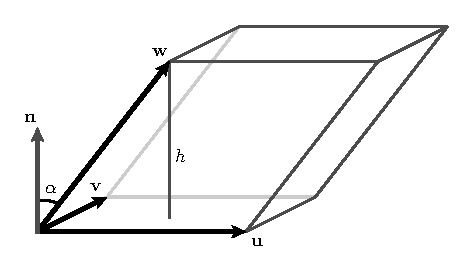
\includegraphics{figures/fig_9_4_volume.eps}
    \caption{The parallelepiped determined by $\vu$, $\vv$, and $\vw$}
    \label{F:9.4.volume}
  \end{center}
\end{figure}

The volume of the parallelepiped is determined by multiplying $A$, the
area of the base, by the height $h$.  As we have just seen, the area
of the base is $|\vu\times\vv|$.  Moreover, the height
$h=|\vw|\cos\alpha$ where $\alpha$ is the angle between $\vw$ and the
vector $\vn$, which is orthogonal to the plane formed by $\vu$ and
$\vv$.  Since $\vn$ is parallel to $\vu\times\vv$, the angle between
$\vw$ and $\vu\times\vv$ is also $\alpha$.  This shows that
$$
|(\vu\times\vv)\cdot\vw| = |\vu\times\vw||\vw|\cos\alpha = Ah,
$$
and therefore 

\vspace*{5pt}
\nin \framebox{\hspace*{3 pt}
\parbox{6.25 in}{
  The volume of the parallelepiped determined by $\vu$, $\vv$, and
  $\vw$ is $|(\vu\times\vv)\cdot\vw|$.
}
\hspace*{3 pt}}
\vspace*{5pt}

The quantity $|(\vu \times
  \vv) \cdot \vw|$ is sometimes called the \emph{scalar triple product}.
  
  \bigskip
  
\begin{activity} \label{A:9.4.6}  Suppose 
  $\vu = \langle 3, 5, -1\rangle$ and $\vv = \langle 2, -2, 1\rangle$.

  \ba
  \item Find two unit vectors orthogonal to both $\vu$ and $\vv$.

  \item Find the volume of the parallelepiped formed by the
    vectors $\vu$, $\vv$, and $\vw = \langle 3,3,1\rangle$.  
    
  \item Find a vector orthogonal to the plane containing the points
    $(0,1,2)$, $(4,1,0)$, and $(-2,2,2)$.

  \item Given the vectors
    $\vu$ and $\vv$ shown below in Figure \ref{F:9.4.activity.2},
    sketch the cross products $\vu\times\vv$ and $\vv\times\vu$.

    \begin{figure}[ht]
      \begin{center}
        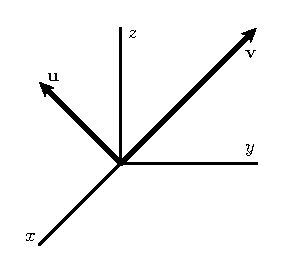
\includegraphics{figures/fig_9_4_activity_2}
        \caption{Vectors $\vu$ and $\vv$}
        \label{F:9.4.activity.2}
      \end{center}
    \end{figure}

  \item Do the vectors $\va = \langle 1,3,-2\rangle$,
    $\vb=\langle2,1,-4\rangle$, and $\vc=\langle 0, 1, 0\rangle$ lie
    in the same plane?  Use the concepts from this section to explain.
    
    \ea
\end{activity}

\begin{activitySolution}
\ba
\item The vector $\vu \times \vv$ is orthogonal to $\vu$ and $\vv$. Now
\[\vu \times \vv = \langle 3, 5, -1\rangle \times \langle 2, -2, 1\rangle = \langle 3, -5, -16 \rangle,\]
so one unit vector orthogonal to $\vu$ and $\vv$ is 
\[\vz=\frac{1}{|\vu \times \vv|} \vu \times \vv = \frac{1}{\sqrt{290}} \langle 3, -5, -16 \rangle.\]
Another unit vector orthogonal to $\vu$ and $\vv$ is $-\vz$. 

\item The volume of the parallelepiped formed by the $\vu$, $\vv$, and $\vw$ is
\[|(\vu \times \vv)\cdot \vw| = |\langle 3, -5, -16 \rangle \cdot \langle 3,3,1\rangle| = 22.\]

\item Let $P=(0,1,2)$, $Q=(4,1,0)$, and $R=(-2,2,2)$. Two vectors in the plane are $\overrightarrow{PQ} = \langle 4,0,-2 \rangle$ and $\overrightarrow{PR} = \langle -2,1,0 \rangle$. So the vector $\overrightarrow{PQ} \times \overrightarrow{PR} = \langle 2, 0, 4\rangle$ is a vector orthogonal to the plane containing the points.

\item Recall that $\vu \times \vv$ is orthogonal to $\vu$ and $\vv$ and that $\vu$, $\vv$ and $\vu \times \vv$ in that order form a right hand system. 

\item Note that $\vu \times \vv = \langle -10, 0, -5 \rangle$, and that $\vu \times \vv$ is orthogonal to every vector in the plane determined by $\vu$ and $\vv$. Now $(\vu \times \vv) \cdot \vw = 0$, so $\vw$ is in the plane determined by $\vu$ and $\vv$.  

\ea
\end{activitySolution}
\aftera


\subsection*{Torque is measured by a cross product}

We have seen that the cross product enables us to produce a vector
perpendicular to two given vectors, to measure the area of a
parallelogram, and to measure the volume of a parallelepiped.  Besides
these geometric applications, the cross product also enables us to
describe a physical quantity called {\em torque}.

Suppose that we would like to turn a bolt using a wrench as shown
in Figure \ref{F:9.4.wrench}.  If a force $\vF$ is applied to the
wrench and $\vr$ is the vector from the position on the wrench at which the force is applied to center of the bolt, we define the
torque, $\tau$, to be
$$
\tau=\vF\times\vr.
$$

\begin{figure}
  \begin{center}
    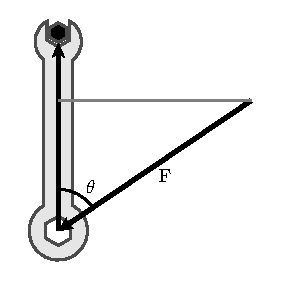
\includegraphics{figures/fig_9_4_wrench.eps}
    \caption{A force applied to a wrench}
    \label{F:9.4.wrench}
  \end{center}
\end{figure}

When a force is applied to an object, Newton's Second Law tells us
that the force is equal to the rate of change of the object's linear
momentum.  Similarly, the torque applied to an object is equal to the
rate of change of the object's angular momentum.  In other words,
torque will cause the bolt to rotate.

In many industrial applications, bolts are required to be tightened
using a specified torque.  Of course, the magnitude of the torque is
$|\tau| =|\vF\times\vr|=|\vF||\vr||\sin(\theta)$.  Thus, to produce a
larger torque, we can increase either $|\vF|$ or $|\vr|$, which you
may know if you have ever removed lug nuts when changing a flat tire.
The ancient Greek mathematician Archimedes said: ``Give me a lever
long enough and a fulcrum on which to place it, and I shall move the
world.''  A modern spin on this statement is: ``Allow me to make
$|\vr|$ large enough, and I shall produce a torque large enough to
move the world.''

\subsection*{Comparing the dot and cross products}

Finally, it is worthwhile to compare and contrast the dot and cross
products.

\begin{itemize}
  \item[(a)] $\vu\cdot\vv$ is a scalar, while $\vu\times\vv$ is a vector.
  \item[(b)] $\vu\cdot\vv = \vv\cdot\vu$, while $\vu\times\vv = -\vv\times\vu$
  \item[(c)] $\vu\cdot\vv = |\vu||\vv|\cos\theta$, while 
    $|\vu\times\vv| = |\vu||\vv|\sin\theta$.
  \item[(d)] $\vu\cdot\vv = 0$ if $\vu$ and $\vv$ are perpendicular, while
    $\vu\times\vv = \vzero$ if $\vu$ and $\vv$ are parallel.
\end{itemize}

\begin{summary}
\item The cross product is defined \emph{only} for vectors in
  $\R^3$. The cross product of vectors $\vu$ and $\vv$ in $\R^3$ is
  the vector
\[(u_1 \vi + u_2 \vj + u_3 \vk) \times (v_1 \vi + v_2 \vj + v_3 \vk) =
(u_2v_3-u_3v_2) \vi - (u_1v_3 - u_3v_1) \vj + (u_1v_2 - u_2v_1) \vk.\]

\item Geometrically, the cross product is
\[\vu \times \vv = |\vu| \ |\vv| \ \sin(\theta) \ \vn,\]
where $\theta$ is the angle between $\vu$ and $\vv$ and $\vn$ is a
unit vector perpendicular to both $\vu$ and $\vv$ as determined by the
right-hand rule.

\item The cross product of vectors $\vu$ and $\vv$ is a vector
  perpendicular to both $\vu$ and $\vv$. 

\item The magnitude $|\vu \times \vv|$ of the cross product of the
  vectors $\vu$ and $\vv$ gives the area of the parallelogram
  determined by $\vu$ and $\vv$. Also, 
  the scalar triple product $|(\vu \times
  \vv) \cdot \vw|$ gives the volume of the parallelepiped determined by
  $\vu$, $\vv$, and $\vw$.
\end{summary}




\nin \hrulefill

\begin{exercises} 

\item \label{Ez:9.4.1}    Let $\vu = 2\vi + \vj$ and $\vv = \vi + 2\vj$ be vectors in $\R^3$.
    \ba
	    \item Without doing any computations, find a unit vector that is orthogonal to both $\vu$ and $\vv$.  What does this tell you about the formula for $\vu \times \vv$?
	    \item Using the bilinearity of the cross product and what you know about cross products involving the fundamental vectors $\vi$ and $\vj$, compute $\vu \times \vv$.
	    \item Next, use the determinant version of Equation~\eqref{E:9.4.cross.def} to compute $\vu \times \vv$.  Write one sentence that compares your results in (a), (b), and (c).
	    \item Find the area of the parallelogram determined by $\vu$ and $\vv$.
    \ea

\begin{exerciseSolution}
    \ba
	    \item Since $\vu$ and $\vv$ lie in the $x$-$y$ plane, the vector $\vk$ is orthogonal to both. So $\vu \times \vv$ is a multiple of $\vk$. 
	    \item The properties of the cross product tell us that 
\begin{align*}
\vu \times \vv &= (2\vi + \vj) \times (\vi + 2\vj) \\
	&= 2(\vi \times \vi) + (\vj \times \vi) + 4(\vi \times \vj) + 2(\vj \times \vj) \\
	&= 2(\vi \times \vi) - (\vi \times \vj) + 4(\vi \times \vj) + 2(\vj \times \vj) \\
	&= 2(\vi \times \vi)  + 3(\vi \times \vj) + 2(\vj \times \vj) \\
	&= 2\vzero + 3\vk + 2\vzero \\
	&= 3 \vk.
\end{align*}
	    \item Using the determinant version of $\vu \times \vv$ we find that 
\[\left| \begin{array}{ccc} \vi & \vj & \vk \\ 2 & 1 & 0 \\ 1 & 2 & 0 \end{array} \right| = [(2)(0)-(0)(1)]\vi - [(1)(0)-(0)(2)] \vj + [(2)(2)-(1)(1)] \vk = 3 \vk.\]
The vectors $\vu$ and $\vv$ lie in the $x$-$y$ plane and a unit vector that is orthogonal to both $\vu$ and $\vv$ is $3 \vk$, established though the determinant formula for the cross product and through the properties of the cross product. 
	    \item The area of the parallelogram determined by $\vu$ and $\vv$ is 
	    \[|\vu \times \vv| = |3\vk| = 3.\]
    \ea
\end{exerciseSolution}

\item \label{Ez:9.4.2}  Let $\vx = \langle 1, 1, 1 \rangle$ and $\vy = \langle 0, 3, -2 \rangle$. 

    \ba
    	\item Are $\vx$ and $\vy$ orthogonal?  Are $\vx$ and $\vy$ parallel?  Clearly explain how you know, using appropriate vector products.
	\item Find a unit vector that is orthogonal to both $\vx$ and $\vy$.
	\item Express $\vy$ as the sum of two vectors:  one parallel to $\vx$, the other orthogonal to $\vx$.
	\item Determine the area of the parallelogram formed by $\vx$ and $\vy$.
    \ea

\begin{exerciseSolution}
  \ba
    \item Two vectors are orthogonal if their dot product is 0. Since $\vx \cdot \vy = 1$, the vectors $\vx$ and $\vy$ are not orthogonal. Vectors $\vx$ and $\vy$ are parallel if one is a scalar multiple of the other, or if their cross product is $\vzero$. Since $\vx \times \vy = -5\vi + 2\vj + 3\vk$, the vectors $\vx$ and $\vy$ are not parallel. 
	\item The vector $\vx \times \vy = -5\vi + 2\vj + 3\vk$ is orthogonal to both $\vx$ and $\vy$, so a unit vector that is orthogonal to both $\vx$ and $\vy$ is $\frac{1}{|\vx \times \vy|} \vx \times \vy = \frac{1}{\sqrt{38}}\langle -5, 2, 3\rangle$. 
	\item The projection 
\[\proj_{\vx} \vy = \frac{\vy \cdot \vx}{\vx \cdot \vx} \vx = \frac{1}{\sqrt{3}}\langle 1,1,1 \rangle\]
of $\vy$ onto $\vx$ is a vector that is parallel to $\vx$, while the vector 
\[\vy - \proj_{\vx} \vy = \frac{1}{\sqrt{3}}\langle -1, 3\sqrt{3}-1, -2\sqrt{3}-1 \rangle\]
is orthogonal to $\vx$. Note that $\vy = \proj_{\vx} \vy + (\vy - \proj_{\vx} \vy)$. 
	\item The area of the parallelogram determined by $\vu$ and $\vv$ is 
	    \[|\vu \times \vv| = | -5\vi + 2\vj + 3\vk| = \sqrt{38}.\]
    \ea
\end{exerciseSolution}

\item \label{Ez:9.4.3}  Consider the triangle in $\R^3$ formed by $P(3, 2, -1)$, $Q(1, -2, 4)$, and $R(4, 4, 0)$.  
%Let $\va = \langle 2, -1, 1 \rangle$ and $\vb = \langle 1, 1, 3 \rangle$.

	\ba
		\item Find $\overrightarrow{PQ}$ and $\overrightarrow{PR}$.
		\item Observe that the area of $\triangle PQR$ is half of the area of the parallelogram formed by $\overrightarrow{PQ}$ and $\overrightarrow{PR}$.  Hence find the area of $\triangle PQR$.
		\item Find a unit vector that is orthogonal to the plane that contains points $P$, $Q$, and $R$.
		\item Determine the measure of $\angle PQR$.
	\ea



\begin{exerciseSolution}
\ba
		\item With the given points $P$, $Q$, and $R$ we have 
\[\overrightarrow{PQ} = \langle -2, -4, 5\rangle  \text{ and } \overrightarrow{PR} = \langle 1, 2, 1 \rangle.\]
		\item The area of the parallelogram formed by $\overrightarrow{PQ}$ and $\overrightarrow{PR}$ is
\[|\overrightarrow{PQ} \times \overrightarrow{PR}| = |\langle -14, 7, 0 \rangle | = \sqrt{245}.\]
Hence the area of $\triangle PQR$ is $\frac{\sqrt{245}}{2}$.
		\item The cross product $\overrightarrow{PQ} \times \overrightarrow{PR}$ is orthogonal to the plane containing $P$, $Q$, and $R$, so a  unit vector that is orthogonal to the plane that contains points $P$, $Q$, and $R$ is 
\[\frac{1}{|\overrightarrow{PQ} \times \overrightarrow{PR}|} \overrightarrow{PQ} \times \overrightarrow{PR} = \frac{1}{\sqrt{245}} \langle -14, 7, 0 \rangle.\]
		\item If $\theta$ is the measure of $\angle PQR$, then 
		\begin{align*}
\theta &= \cos^{-1}\left(\frac{\overrightarrow{QP} \cdot \overrightarrow{QR}}{|\overrightarrow{QP}| |\overrightarrow{QR}|} \right) \\
	&= \cos^{-1}\left(\frac{\langle 2, 4, -5 \rangle \cdot \langle 3, 6, -4 \rangle}{|\langle 2, 4, -5 \rangle| |\langle 3, 6, -4 \rangle|} \right)\\
	&= \cos^{-1}\left(\frac{50}{\sqrt{45} \sqrt{61}} \right) \\
	&\approx 17.38^{\circ}.
\end{align*} 
	\ea
\end{exerciseSolution}



%\item \label{Ez:9.3.1}   

%A tetrahedron is a four-sided solid in $\R^3$, each of whose faces are triangles.  Consider the tetrahedron whose vertices are the points $(1,0,0)$, $(0,1,0)$, $(1,0,0)$, and $(1,1,1)$ as shown in Figure
%\begin{figure}[ht]
%\begin{center}
 %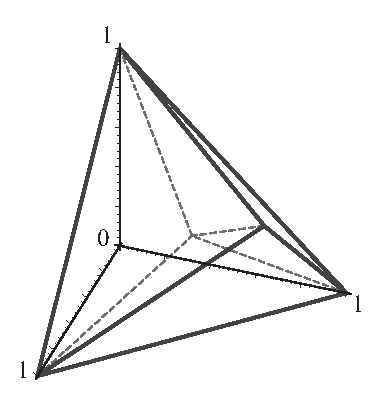
\includegraphics{figures/9_3_Ez1_tetrahedron.eps}
% \caption{The tetrahedron with vertices $(1,0,0)$, $(0,1,0)$, $(1,0,0)$, and $(1,1,1)$.} \label{F:9_3_Ez1_tetrahedron}
%\end{center}
%\end{figure}
%The \emph{centroid} of the tetrahedron is the average of the four vertices, which is the point $(\frac{1}{2}, \frac{1}{2}, \frac{1}{2})$, as shown at the intersection of the dotted lines.
 %   \ba
  %  	\item Consider the face determined by $(1,0,0)$, $(1,1,1)$, and $(0,0,1)$.  Explain why this face is an equilateral triangle.
%	\item 
 %   \ea

%\begin{exerciseSolution}
%\end{exerciseSolution}

\end{exercises}
\afterexercises


\clearpage

